\documentclass[1p]{elsarticle_modified}
%\bibliographystyle{elsarticle-num}

%\usepackage[colorlinks]{hyperref}
%\usepackage{abbrmath_seonhwa} %\Abb, \Ascr, \Acal ,\Abf, \Afrak
\usepackage{amsfonts}
\usepackage{amssymb}
\usepackage{amsmath}
\usepackage{amsthm}
\usepackage{scalefnt}
\usepackage{amsbsy}
\usepackage{kotex}
\usepackage{caption}
\usepackage{subfig}
\usepackage{color}
\usepackage{graphicx}
\usepackage{xcolor} %% white, black, red, green, blue, cyan, magenta, yellow
\usepackage{float}
\usepackage{setspace}
\usepackage{hyperref}

\usepackage{tikz}
\usetikzlibrary{arrows}

\usepackage{multirow}
\usepackage{array} % fixed length table
\usepackage{hhline}

%%%%%%%%%%%%%%%%%%%%%
\makeatletter
\renewcommand*\env@matrix[1][\arraystretch]{%
	\edef\arraystretch{#1}%
	\hskip -\arraycolsep
	\let\@ifnextchar\new@ifnextchar
	\array{*\c@MaxMatrixCols c}}
\makeatother %https://tex.stackexchange.com/questions/14071/how-can-i-increase-the-line-spacing-in-a-matrix
%%%%%%%%%%%%%%%

\usepackage[normalem]{ulem}

\newcommand{\msout}[1]{\ifmmode\text{\sout{\ensuremath{#1}}}\else\sout{#1}\fi}
%SOURCE: \msout is \stkout macro in https://tex.stackexchange.com/questions/20609/strikeout-in-math-mode

\newcommand{\cancel}[1]{
	\ifmmode
	{\color{red}\msout{#1}}
	\else
	{\color{red}\sout{#1}}
	\fi
}

\newcommand{\add}[1]{
	{\color{blue}\uwave{#1}}
}

\newcommand{\replace}[2]{
	\ifmmode
	{\color{red}\msout{#1}}{\color{blue}\uwave{#2}}
	\else
	{\color{red}\sout{#1}}{\color{blue}\uwave{#2}}
	\fi
}

\newcommand{\Sol}{\mathcal{S}} %segment
\newcommand{\D}{D} %diagram
\newcommand{\A}{\mathcal{A}} %arc


%%%%%%%%%%%%%%%%%%%%%%%%%%%%%5 test

\def\sl{\operatorname{\textup{SL}}(2,\Cbb)}
\def\psl{\operatorname{\textup{PSL}}(2,\Cbb)}
\def\quan{\mkern 1mu \triangleright \mkern 1mu}

\theoremstyle{definition}
\newtheorem{thm}{Theorem}[section]
\newtheorem{prop}[thm]{Proposition}
\newtheorem{lem}[thm]{Lemma}
\newtheorem{ques}[thm]{Question}
\newtheorem{cor}[thm]{Corollary}
\newtheorem{defn}[thm]{Definition}
\newtheorem{exam}[thm]{Example}
\newtheorem{rmk}[thm]{Remark}
\newtheorem{alg}[thm]{Algorithm}

\newcommand{\I}{\sqrt{-1}}
\begin{document}

%\begin{frontmatter}
%
%\title{Boundary parabolic representations of knots up to 8 crossings}
%
%%% Group authors per affiliation:
%\author{Yunhi Cho} 
%\address{Department of Mathematics, University of Seoul, Seoul, Korea}
%\ead{yhcho@uos.ac.kr}
%
%
%\author{Seonhwa Kim} %\fnref{s_kim}}
%\address{Center for Geometry and Physics, Institute for Basic Science, Pohang, 37673, Korea}
%\ead{ryeona17@ibs.re.kr}
%
%\author{Hyuk Kim}
%\address{Department of Mathematical Sciences, Seoul National University, Seoul 08826, Korea}
%\ead{hyukkim@snu.ac.kr}
%
%\author{Seokbeom Yoon}
%\address{Department of Mathematical Sciences, Seoul National University, Seoul, 08826,  Korea}
%\ead{sbyoon15@snu.ac.kr}
%
%\begin{abstract}
%We find all boundary parabolic representation of knots up to 8 crossings.
%
%\end{abstract}
%\begin{keyword}
%    \MSC[2010] 57M25 
%\end{keyword}
%
%\end{frontmatter}

%\linenumbers
%\tableofcontents
%
\newcommand\colored[1]{\textcolor{white}{\rule[-0.35ex]{0.8em}{1.4ex}}\kern-0.8em\color{red} #1}%
%\newcommand\colored[1]{\textcolor{white}{ #1}\kern-2.17ex	\textcolor{white}{ #1}\kern-1.81ex	\textcolor{white}{ #1}\kern-2.15ex\color{red}#1	}

{\Large $\underline{11n_{160}~(K11n_{160})}$}

\setlength{\tabcolsep}{10pt}
\renewcommand{\arraystretch}{1.6}
\vspace{1cm}\begin{tabular}{m{100pt}>{\centering\arraybackslash}m{274pt}}
\multirow{5}{120pt}{
	\centering
	\includegraphics[width=112pt]{../../../GIT/diagram.site/Diagrams/png/776_11n_160.png}\\
\ \ \ A knot diagram\footnotemark}&
\allowdisplaybreaks
\textbf{Linearized knot diagam} \\
\cline{2-2}
 &
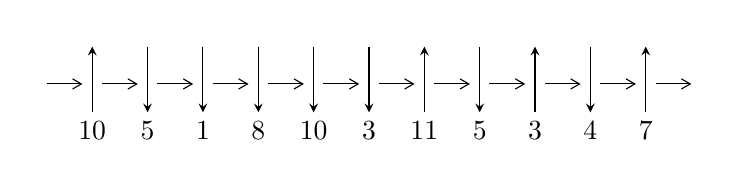
\begin{tikzpicture}[x=20pt, y=17pt]
	% nodes
	\node (C0) at (0, 0) {};
	\node (C1) at (1, 0) {};
	\node (C1U) at (1, +1) {};
	\node (C1D) at (1, -1) {10};

	\node (C2) at (2, 0) {};
	\node (C2U) at (2, +1) {};
	\node (C2D) at (2, -1) {5};

	\node (C3) at (3, 0) {};
	\node (C3U) at (3, +1) {};
	\node (C3D) at (3, -1) {1};

	\node (C4) at (4, 0) {};
	\node (C4U) at (4, +1) {};
	\node (C4D) at (4, -1) {8};

	\node (C5) at (5, 0) {};
	\node (C5U) at (5, +1) {};
	\node (C5D) at (5, -1) {10};

	\node (C6) at (6, 0) {};
	\node (C6U) at (6, +1) {};
	\node (C6D) at (6, -1) {3};

	\node (C7) at (7, 0) {};
	\node (C7U) at (7, +1) {};
	\node (C7D) at (7, -1) {11};

	\node (C8) at (8, 0) {};
	\node (C8U) at (8, +1) {};
	\node (C8D) at (8, -1) {5};

	\node (C9) at (9, 0) {};
	\node (C9U) at (9, +1) {};
	\node (C9D) at (9, -1) {3};

	\node (C10) at (10, 0) {};
	\node (C10U) at (10, +1) {};
	\node (C10D) at (10, -1) {4};

	\node (C11) at (11, 0) {};
	\node (C11U) at (11, +1) {};
	\node (C11D) at (11, -1) {7};
	\node (C12) at (12, 0) {};

	% arrows
	\draw[->,>={angle 60}]
	(C0) edge (C1) (C1) edge (C2) (C2) edge (C3) (C3) edge (C4) (C4) edge (C5) (C5) edge (C6) (C6) edge (C7) (C7) edge (C8) (C8) edge (C9) (C9) edge (C10) (C10) edge (C11) (C11) edge (C12) ;	\draw[->,>=stealth]
	(C1D) edge (C1U) (C2U) edge (C2D) (C3U) edge (C3D) (C4U) edge (C4D) (C5U) edge (C5D) (C6U) edge (C6D) (C7D) edge (C7U) (C8U) edge (C8D) (C9D) edge (C9U) (C10U) edge (C10D) (C11D) edge (C11U) ;
	\end{tikzpicture} \\
\hhline{~~} \\& 
\textbf{Solving Sequence} \\ \cline{2-2} 
 &
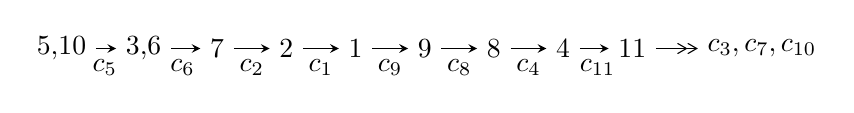
\begin{tikzpicture}[x=25pt, y=7pt]
	% node
	\node (A0) at (-1/8, 0) {5,10};
	\node (A1) at (17/16, 0) {3,6};
	\node (A2) at (17/8, 0) {7};
	\node (A3) at (25/8, 0) {2};
	\node (A4) at (33/8, 0) {1};
	\node (A5) at (41/8, 0) {9};
	\node (A6) at (49/8, 0) {8};
	\node (A7) at (57/8, 0) {4};
	\node (A8) at (65/8, 0) {11};
	\node (C1) at (1/2, -1) {$c_{5}$};
	\node (C2) at (13/8, -1) {$c_{6}$};
	\node (C3) at (21/8, -1) {$c_{2}$};
	\node (C4) at (29/8, -1) {$c_{1}$};
	\node (C5) at (37/8, -1) {$c_{9}$};
	\node (C6) at (45/8, -1) {$c_{8}$};
	\node (C7) at (53/8, -1) {$c_{4}$};
	\node (C8) at (61/8, -1) {$c_{11}$};
	\node (A9) at (10, 0) {$c_{3},c_{7},c_{10}$};

	% edge
	\draw[->,>=stealth]	
	(A0) edge (A1) (A1) edge (A2) (A2) edge (A3) (A3) edge (A4) (A4) edge (A5) (A5) edge (A6) (A6) edge (A7) (A7) edge (A8) ;
	\draw[->>,>={angle 60}]	
	(A8) edge (A9);
\end{tikzpicture} \\ 

\end{tabular} \\

\footnotetext{
The image of knot diagram is generated by the software ``\textbf{Draw programme}" developed by Andrew Bartholomew(\url{http://www.layer8.co.uk/maths/draw/index.htm\#Running-draw}), where we modified some parts for our purpose(\url{https://github.com/CATsTAILs/LinksPainter}).
}\phantom \\ \newline 
\centering \textbf{Ideals for irreducible components\footnotemark of $X_{\text{par}}$} 
 
\begin{align*}
I^u_{1}&=\langle 
-2.61154\times10^{116} u^{41}+7.44138\times10^{116} u^{40}+\cdots+2.20130\times10^{118} b+2.20567\times10^{118},\\
\phantom{I^u_{1}}&\phantom{= \langle  }2.76575\times10^{118} u^{41}-8.73496\times10^{118} u^{40}+\cdots+2.42143\times10^{119} a+9.10967\times10^{119},\\
\phantom{I^u_{1}}&\phantom{= \langle  }u^{42}-3 u^{41}+\cdots-184 u-11\rangle \\
I^u_{2}&=\langle 
31 u^8+26 u^7+50 u^6+165 u^5-26 u^4-204 u^3-34 u^2+47 b+86 u+75,\\
\phantom{I^u_{2}}&\phantom{= \langle  }34 u^8+27 u^7+23 u^6+184 u^5-74 u^4-342 u^3+131 u^2+47 a+158 u-83,\\
\phantom{I^u_{2}}&\phantom{= \langle  }u^9+2 u^8+2 u^7+7 u^6+5 u^5-10 u^4-6 u^3+6 u^2+3 u+1\rangle \\
\\
\end{align*}
\raggedright * 2 irreducible components of $\dim_{\mathbb{C}}=0$, with total 51 representations.\\
\footnotetext{All coefficients of polynomials are rational numbers. But the coefficients are sometimes approximated in decimal forms when there is not enough margin.}
\newpage
\renewcommand{\arraystretch}{1}
\centering \section*{I. $I^u_{1}= \langle -2.61\times10^{116} u^{41}+7.44\times10^{116} u^{40}+\cdots+2.20\times10^{118} b+2.21\times10^{118},\;2.77\times10^{118} u^{41}-8.73\times10^{118} u^{40}+\cdots+2.42\times10^{119} a+9.11\times10^{119},\;u^{42}-3 u^{41}+\cdots-184 u-11 \rangle$}
\flushleft \textbf{(i) Arc colorings}\\
\begin{tabular}{m{7pt} m{180pt} m{7pt} m{180pt} }
\flushright $a_{5}=$&$\begin{pmatrix}1\\0\end{pmatrix}$ \\
\flushright $a_{10}=$&$\begin{pmatrix}0\\u\end{pmatrix}$ \\
\flushright $a_{3}=$&$\begin{pmatrix}-0.114220 u^{41}+0.360736 u^{40}+\cdots+116.228 u-3.76211\\0.0118637 u^{41}-0.0338046 u^{40}+\cdots-14.7028 u-1.00199\end{pmatrix}$ \\
\flushright $a_{6}=$&$\begin{pmatrix}1\\u^2\end{pmatrix}$ \\
\flushright $a_{7}=$&$\begin{pmatrix}-0.0851467 u^{41}+0.256373 u^{40}+\cdots+160.031 u+16.8852\\-0.0100801 u^{41}+0.0314357 u^{40}+\cdots+4.32560 u-0.298656\end{pmatrix}$ \\
\flushright $a_{2}=$&$\begin{pmatrix}-0.102356 u^{41}+0.326932 u^{40}+\cdots+101.525 u-4.76410\\0.0118637 u^{41}-0.0338046 u^{40}+\cdots-14.7028 u-1.00199\end{pmatrix}$ \\
\flushright $a_{1}=$&$\begin{pmatrix}-0.102356 u^{41}+0.326932 u^{40}+\cdots+101.525 u-4.76410\\0.00934866 u^{41}-0.0266415 u^{40}+\cdots-12.1739 u-0.783495\end{pmatrix}$ \\
\flushright $a_{9}=$&$\begin{pmatrix}0.183123 u^{41}-0.552897 u^{40}+\cdots-292.420 u-21.2506\\-0.00244803 u^{41}+0.00733234 u^{40}+\cdots+2.14687 u+0.897796\end{pmatrix}$ \\
\flushright $a_{8}=$&$\begin{pmatrix}0.180675 u^{41}-0.545564 u^{40}+\cdots-290.273 u-20.3528\\-0.00244803 u^{41}+0.00733234 u^{40}+\cdots+2.14687 u+0.897796\end{pmatrix}$ \\
\flushright $a_{4}=$&$\begin{pmatrix}-0.157339 u^{41}+0.476272 u^{40}+\cdots+234.882 u+15.0129\\0.00294723 u^{41}-0.0113162 u^{40}+\cdots-3.44539 u-0.785309\end{pmatrix}$ \\
\flushright $a_{11}=$&$\begin{pmatrix}-0.149328 u^{41}+0.463397 u^{40}+\cdots+205.737 u+5.85422\\0.00974472 u^{41}-0.0271814 u^{40}+\cdots-13.4504 u-1.21086\end{pmatrix}$\\ \flushright $a_{11}=$&$\begin{pmatrix}-0.149328 u^{41}+0.463397 u^{40}+\cdots+205.737 u+5.85422\\0.00974472 u^{41}-0.0271814 u^{40}+\cdots-13.4504 u-1.21086\end{pmatrix}$\\&\end{tabular}
\flushleft \textbf{(ii) Obstruction class $= -1$}\\~\\
\flushleft \textbf{(iii) Cusp Shapes $= -0.0407139 u^{41}+0.122846 u^{40}+\cdots+94.2507 u+5.40926$}\\~\\
\newpage\renewcommand{\arraystretch}{1}
\flushleft \textbf{(iv) u-Polynomials at the component}\newline \\
\begin{tabular}{m{50pt}|m{274pt}}
Crossings & \hspace{64pt}u-Polynomials at each crossing \\
\hline $$\begin{aligned}c_{1}\end{aligned}$$&$\begin{aligned}
&u^{42}+2 u^{41}+\cdots-124 u-4
\end{aligned}$\\
\hline $$\begin{aligned}c_{2}\end{aligned}$$&$\begin{aligned}
&u^{42}+20 u^{40}+\cdots-749 u-101
\end{aligned}$\\
\hline $$\begin{aligned}c_{3}\end{aligned}$$&$\begin{aligned}
&u^{42}-6 u^{41}+\cdots-8 u+1
\end{aligned}$\\
\hline $$\begin{aligned}c_{4},c_{8}\end{aligned}$$&$\begin{aligned}
&u^{42}+2 u^{41}+\cdots+556 u+116
\end{aligned}$\\
\hline $$\begin{aligned}c_{5}\end{aligned}$$&$\begin{aligned}
&u^{42}-3 u^{41}+\cdots-184 u-11
\end{aligned}$\\
\hline $$\begin{aligned}c_{6}\end{aligned}$$&$\begin{aligned}
&u^{42}+u^{40}+\cdots+106 u-97
\end{aligned}$\\
\hline $$\begin{aligned}c_{7},c_{11}\end{aligned}$$&$\begin{aligned}
&u^{42}-4 u^{41}+\cdots-47 u-13
\end{aligned}$\\
\hline $$\begin{aligned}c_{9}\end{aligned}$$&$\begin{aligned}
&u^{42}- u^{41}+\cdots+112 u-23
\end{aligned}$\\
\hline $$\begin{aligned}c_{10}\end{aligned}$$&$\begin{aligned}
&u^{42}+2 u^{41}+\cdots+128 u+29
\end{aligned}$\\
\hline
\end{tabular}\\~\\
\newpage\renewcommand{\arraystretch}{1}
\flushleft \textbf{(v) Riley Polynomials at the component}\newline \\
\begin{tabular}{m{50pt}|m{274pt}}
Crossings & \hspace{64pt}Riley Polynomials at each crossing \\
\hline $$\begin{aligned}c_{1}\end{aligned}$$&$\begin{aligned}
&y^{42}-72 y^{41}+\cdots-5760 y+16
\end{aligned}$\\
\hline $$\begin{aligned}c_{2}\end{aligned}$$&$\begin{aligned}
&y^{42}+40 y^{41}+\cdots+72673 y+10201
\end{aligned}$\\
\hline $$\begin{aligned}c_{3}\end{aligned}$$&$\begin{aligned}
&y^{42}+4 y^{41}+\cdots-30 y+1
\end{aligned}$\\
\hline $$\begin{aligned}c_{4},c_{8}\end{aligned}$$&$\begin{aligned}
&y^{42}-24 y^{41}+\cdots-45120 y+13456
\end{aligned}$\\
\hline $$\begin{aligned}c_{5}\end{aligned}$$&$\begin{aligned}
&y^{42}+51 y^{41}+\cdots+5722 y+121
\end{aligned}$\\
\hline $$\begin{aligned}c_{6}\end{aligned}$$&$\begin{aligned}
&y^{42}+2 y^{41}+\cdots+164916 y+9409
\end{aligned}$\\
\hline $$\begin{aligned}c_{7},c_{11}\end{aligned}$$&$\begin{aligned}
&y^{42}+26 y^{41}+\cdots-805 y+169
\end{aligned}$\\
\hline $$\begin{aligned}c_{9}\end{aligned}$$&$\begin{aligned}
&y^{42}-45 y^{41}+\cdots-1274 y+529
\end{aligned}$\\
\hline $$\begin{aligned}c_{10}\end{aligned}$$&$\begin{aligned}
&y^{42}-12 y^{41}+\cdots-22358 y+841
\end{aligned}$\\
\hline
\end{tabular}\\~\\
\newpage\flushleft \textbf{(vi) Complex Volumes and Cusp Shapes}
$$\begin{array}{c|c|c}  
\text{Solutions to }I^u_{1}& \I (\text{vol} + \sqrt{-1}CS) & \text{Cusp shape}\\
 \hline 
\begin{aligned}
u &= \phantom{-}0.838508 + 0.288184 I \\
a &= \phantom{-}1.170650 + 0.251577 I \\
b &= -0.474707 + 0.528975 I\end{aligned}
 & -3.52003 + 2.03312 I & -8.42216 - 3.37678 I \\ \hline\begin{aligned}
u &= \phantom{-}0.838508 - 0.288184 I \\
a &= \phantom{-}1.170650 - 0.251577 I \\
b &= -0.474707 - 0.528975 I\end{aligned}
 & -3.52003 - 2.03312 I & -8.42216 + 3.37678 I \\ \hline\begin{aligned}
u &= -1.192800 + 0.009739 I \\
a &= -0.0763919 + 0.0920066 I \\
b &= -0.593548 + 0.597226 I\end{aligned}
 & -1.94227 - 0.55855 I & -3.25163 - 2.41810 I \\ \hline\begin{aligned}
u &= -1.192800 - 0.009739 I \\
a &= -0.0763919 - 0.0920066 I \\
b &= -0.593548 - 0.597226 I\end{aligned}
 & -1.94227 + 0.55855 I & -3.25163 + 2.41810 I \\ \hline\begin{aligned}
u &= -0.394106 + 0.627152 I \\
a &= \phantom{-}1.78252 - 0.23343 I \\
b &= -0.403159 - 0.306921 I\end{aligned}
 & -4.10677 - 1.00823 I & -6.95415 - 0.51830 I \\ \hline\begin{aligned}
u &= -0.394106 - 0.627152 I \\
a &= \phantom{-}1.78252 + 0.23343 I \\
b &= -0.403159 + 0.306921 I\end{aligned}
 & -4.10677 + 1.00823 I & -6.95415 + 0.51830 I \\ \hline\begin{aligned}
u &= -0.549682 + 0.472418 I \\
a &= \phantom{-}0.724998 + 0.076343 I \\
b &= \phantom{-}0.045927 + 0.526713 I\end{aligned}
 & -0.95288 + 2.06296 I & -2.70729 - 3.81916 I \\ \hline\begin{aligned}
u &= -0.549682 - 0.472418 I \\
a &= \phantom{-}0.724998 - 0.076343 I \\
b &= \phantom{-}0.045927 - 0.526713 I\end{aligned}
 & -0.95288 - 2.06296 I & -2.70729 + 3.81916 I \\ \hline\begin{aligned}
u &= \phantom{-}0.071542 + 1.319740 I \\
a &= \phantom{-}0.310251 + 1.197800 I \\
b &= -0.53365 - 1.65271 I\end{aligned}
 & -0.24491 - 5.34601 I & -6.61771 + 6.40608 I \\ \hline\begin{aligned}
u &= \phantom{-}0.071542 - 1.319740 I \\
a &= \phantom{-}0.310251 - 1.197800 I \\
b &= -0.53365 + 1.65271 I\end{aligned}
 & -0.24491 + 5.34601 I & -6.61771 - 6.40608 I\\
 \hline 
 \end{array}$$\newpage$$\begin{array}{c|c|c}  
\text{Solutions to }I^u_{1}& \I (\text{vol} + \sqrt{-1}CS) & \text{Cusp shape}\\
 \hline 
\begin{aligned}
u &= \phantom{-}0.322779 + 0.584470 I \\
a &= -1.96834 - 1.04003 I \\
b &= -0.018310 + 0.894802 I\end{aligned}
 & -4.81718 + 6.58441 I & -5.59437 - 5.87348 I \\ \hline\begin{aligned}
u &= \phantom{-}0.322779 - 0.584470 I \\
a &= -1.96834 + 1.04003 I \\
b &= -0.018310 - 0.894802 I\end{aligned}
 & -4.81718 - 6.58441 I & -5.59437 + 5.87348 I \\ \hline\begin{aligned}
u &= \phantom{-}0.194310 + 0.577382 I \\
a &= \phantom{-}0.904526 - 0.641045 I \\
b &= \phantom{-}0.492771 - 0.001301 I\end{aligned}
 & \phantom{-}0.96120 + 1.37637 I & \phantom{-}2.37205 - 4.71298 I \\ \hline\begin{aligned}
u &= \phantom{-}0.194310 - 0.577382 I \\
a &= \phantom{-}0.904526 + 0.641045 I \\
b &= \phantom{-}0.492771 + 0.001301 I\end{aligned}
 & \phantom{-}0.96120 - 1.37637 I & \phantom{-}2.37205 + 4.71298 I \\ \hline\begin{aligned}
u &= \phantom{-}0.207450 + 0.501375 I \\
a &= \phantom{-}1.094850 - 0.376955 I \\
b &= -1.257640 + 0.545229 I\end{aligned}
 & -4.48395 + 1.62517 I & -2.04474 - 0.35828 I \\ \hline\begin{aligned}
u &= \phantom{-}0.207450 - 0.501375 I \\
a &= \phantom{-}1.094850 + 0.376955 I \\
b &= -1.257640 - 0.545229 I\end{aligned}
 & -4.48395 - 1.62517 I & -2.04474 + 0.35828 I \\ \hline\begin{aligned}
u &= -0.294933 + 0.306279 I \\
a &= \phantom{-}1.39370 + 1.50859 I \\
b &= \phantom{-}1.54579 + 0.18285 I\end{aligned}
 & -5.60720 - 6.66981 I & -4.81384 + 5.61602 I \\ \hline\begin{aligned}
u &= -0.294933 - 0.306279 I \\
a &= \phantom{-}1.39370 - 1.50859 I \\
b &= \phantom{-}1.54579 - 0.18285 I\end{aligned}
 & -5.60720 + 6.66981 I & -4.81384 - 5.61602 I \\ \hline\begin{aligned}
u &= -0.368795\phantom{ +0.000000I} \\
a &= \phantom{-}0.896001\phantom{ +0.000000I} \\
b &= -0.725613\phantom{ +0.000000I}\end{aligned}
 & -1.10908\phantom{ +0.000000I} & -10.5890\phantom{ +0.000000I} \\ \hline\begin{aligned}
u &= -0.45702 + 1.66340 I \\
a &= -0.199299 - 1.049700 I \\
b &= -0.07435 + 1.78893 I\end{aligned}
 & \phantom{-}5.41237 + 6.59053 I & \phantom{-0.000000 } 0\\
 \hline 
 \end{array}$$\newpage$$\begin{array}{c|c|c}  
\text{Solutions to }I^u_{1}& \I (\text{vol} + \sqrt{-1}CS) & \text{Cusp shape}\\
 \hline 
\begin{aligned}
u &= -0.45702 - 1.66340 I \\
a &= -0.199299 + 1.049700 I \\
b &= -0.07435 - 1.78893 I\end{aligned}
 & \phantom{-}5.41237 - 6.59053 I & \phantom{-0.000000 } 0 \\ \hline\begin{aligned}
u &= \phantom{-}1.72020 + 0.21164 I \\
a &= -0.346970 - 0.170035 I \\
b &= -0.301486 + 0.307655 I\end{aligned}
 & -6.74843 - 5.64741 I & \phantom{-0.000000 } 0 \\ \hline\begin{aligned}
u &= \phantom{-}1.72020 - 0.21164 I \\
a &= -0.346970 + 0.170035 I \\
b &= -0.301486 - 0.307655 I\end{aligned}
 & -6.74843 + 5.64741 I & \phantom{-0.000000 } 0 \\ \hline\begin{aligned}
u &= \phantom{-}0.06851 + 1.75165 I \\
a &= \phantom{-}0.208522 - 1.001630 I \\
b &= -0.26966 + 1.44580 I\end{aligned}
 & \phantom{-}4.33527 + 2.92425 I & \phantom{-0.000000 } 0 \\ \hline\begin{aligned}
u &= \phantom{-}0.06851 - 1.75165 I \\
a &= \phantom{-}0.208522 + 1.001630 I \\
b &= -0.26966 - 1.44580 I\end{aligned}
 & \phantom{-}4.33527 - 2.92425 I & \phantom{-0.000000 } 0 \\ \hline\begin{aligned}
u &= \phantom{-}0.42070 + 1.74601 I \\
a &= -0.218861 + 0.855059 I \\
b &= -0.01981 - 1.75119 I\end{aligned}
 & \phantom{-}7.93236 - 2.29439 I & \phantom{-0.000000 } 0 \\ \hline\begin{aligned}
u &= \phantom{-}0.42070 - 1.74601 I \\
a &= -0.218861 - 0.855059 I \\
b &= -0.01981 + 1.75119 I\end{aligned}
 & \phantom{-}7.93236 + 2.29439 I & \phantom{-0.000000 } 0 \\ \hline\begin{aligned}
u &= -0.64354 + 1.75757 I \\
a &= \phantom{-}0.209152 + 0.893674 I \\
b &= -0.301319 - 1.190510 I\end{aligned}
 & \phantom{-}3.08658 + 1.51461 I & \phantom{-0.000000 } 0 \\ \hline\begin{aligned}
u &= -0.64354 - 1.75757 I \\
a &= \phantom{-}0.209152 - 0.893674 I \\
b &= -0.301319 + 1.190510 I\end{aligned}
 & \phantom{-}3.08658 - 1.51461 I & \phantom{-0.000000 } 0 \\ \hline\begin{aligned}
u &= -0.0616260 + 0.0746193 I \\
a &= -10.96120 + 5.34669 I \\
b &= -0.086589 - 0.706593 I\end{aligned}
 & -1.12929 - 2.58933 I & -0.40470 + 5.03166 I\\
 \hline 
 \end{array}$$\newpage$$\begin{array}{c|c|c}  
\text{Solutions to }I^u_{1}& \I (\text{vol} + \sqrt{-1}CS) & \text{Cusp shape}\\
 \hline 
\begin{aligned}
u &= -0.0616260 - 0.0746193 I \\
a &= -10.96120 - 5.34669 I \\
b &= -0.086589 + 0.706593 I\end{aligned}
 & -1.12929 + 2.58933 I & -0.40470 - 5.03166 I \\ \hline\begin{aligned}
u &= -0.17719 + 1.92230 I \\
a &= \phantom{-}0.182597 - 0.970850 I \\
b &= -0.14313 + 1.50275 I\end{aligned}
 & \phantom{-}4.55674 + 2.88338 I & \phantom{-0.000000 } 0 \\ \hline\begin{aligned}
u &= -0.17719 - 1.92230 I \\
a &= \phantom{-}0.182597 + 0.970850 I \\
b &= -0.14313 - 1.50275 I\end{aligned}
 & \phantom{-}4.55674 - 2.88338 I & \phantom{-0.000000 } 0 \\ \hline\begin{aligned}
u &= \phantom{-}0.50851 + 1.89248 I \\
a &= \phantom{-}0.236773 + 0.848855 I \\
b &= -0.08366 - 1.50753 I\end{aligned}
 & \phantom{-}3.06015 - 4.00976 I & \phantom{-0.000000 } 0 \\ \hline\begin{aligned}
u &= \phantom{-}0.50851 - 1.89248 I \\
a &= \phantom{-}0.236773 - 0.848855 I \\
b &= -0.08366 + 1.50753 I\end{aligned}
 & \phantom{-}3.06015 + 4.00976 I & \phantom{-0.000000 } 0 \\ \hline\begin{aligned}
u &= \phantom{-}1.99479\phantom{ +0.000000I} \\
a &= \phantom{-}0.535185\phantom{ +0.000000I} \\
b &= \phantom{-}2.64314\phantom{ +0.000000I}\end{aligned}
 & \phantom{-}0.445368\phantom{ +0.000000I} & \phantom{-0.000000 } 0 \\ \hline\begin{aligned}
u &= -0.41191 + 1.95357 I \\
a &= -0.017188 + 0.836754 I \\
b &= \phantom{-}0.57790 - 1.71570 I\end{aligned}
 & \phantom{-}5.50962 + 8.17142 I & \phantom{-0.000000 } 0 \\ \hline\begin{aligned}
u &= -0.41191 - 1.95357 I \\
a &= -0.017188 - 0.836754 I \\
b &= \phantom{-}0.57790 + 1.71570 I\end{aligned}
 & \phantom{-}5.50962 - 8.17142 I & \phantom{-0.000000 } 0 \\ \hline\begin{aligned}
u &= \phantom{-}0.48329 + 1.95963 I \\
a &= -0.087238 - 0.890319 I \\
b &= \phantom{-}0.52555 + 1.75387 I\end{aligned}
 & \phantom{-}0.9874 - 14.3018 I & \phantom{-0.000000 } 0 \\ \hline\begin{aligned}
u &= \phantom{-}0.48329 - 1.95963 I \\
a &= -0.087238 + 0.890319 I \\
b &= \phantom{-}0.52555 - 1.75387 I\end{aligned}
 & \phantom{-}0.9874 + 14.3018 I & \phantom{-0.000000 } 0\\
 \hline 
 \end{array}$$\newpage$$\begin{array}{c|c|c}  
\text{Solutions to }I^u_{1}& \I (\text{vol} + \sqrt{-1}CS) & \text{Cusp shape}\\
 \hline 
\begin{aligned}
u &= \phantom{-}0.03402 + 2.11235 I \\
a &= -0.104154 - 0.553583 I \\
b &= \phantom{-}0.41431 + 2.06998 I\end{aligned}
 & \phantom{-}0.510430 - 0.864801 I & \phantom{-0.000000 } 0 \\ \hline\begin{aligned}
u &= \phantom{-}0.03402 - 2.11235 I \\
a &= -0.104154 + 0.553583 I \\
b &= \phantom{-}0.41431 - 2.06998 I\end{aligned}
 & \phantom{-}0.510430 + 0.864801 I & \phantom{-0.000000 } 0\\
 \hline 
 \end{array}$$\newpage\newpage\renewcommand{\arraystretch}{1}
\centering \section*{II. $I^u_{2}= \langle 31 u^8+26 u^7+\cdots+47 b+75,\;34 u^8+27 u^7+\cdots+47 a-83,\;u^9+2 u^8+\cdots+3 u+1 \rangle$}
\flushleft \textbf{(i) Arc colorings}\\
\begin{tabular}{m{7pt} m{180pt} m{7pt} m{180pt} }
\flushright $a_{5}=$&$\begin{pmatrix}1\\0\end{pmatrix}$ \\
\flushright $a_{10}=$&$\begin{pmatrix}0\\u\end{pmatrix}$ \\
\flushright $a_{3}=$&$\begin{pmatrix}-0.723404 u^{8}-0.574468 u^{7}+\cdots-3.36170 u+1.76596\\-0.659574 u^{8}-0.553191 u^{7}+\cdots-1.82979 u-1.59574\end{pmatrix}$ \\
\flushright $a_{6}=$&$\begin{pmatrix}1\\u^2\end{pmatrix}$ \\
\flushright $a_{7}=$&$\begin{pmatrix}-0.148936 u^{8}-0.382979 u^{7}+\cdots+0.425532 u-1.48936\\0.872340 u^{8}+0.957447 u^{7}+\cdots+2.93617 u+1.72340\end{pmatrix}$ \\
\flushright $a_{2}=$&$\begin{pmatrix}-1.38298 u^{8}-1.12766 u^{7}+\cdots-5.19149 u+0.170213\\-0.659574 u^{8}-0.553191 u^{7}+\cdots-1.82979 u-1.59574\end{pmatrix}$ \\
\flushright $a_{1}=$&$\begin{pmatrix}-1.38298 u^{8}-1.12766 u^{7}+\cdots-5.19149 u+0.170213\\-2.72340 u^{8}-1.57447 u^{7}+\cdots-5.36170 u-3.23404\end{pmatrix}$ \\
\flushright $a_{9}=$&$\begin{pmatrix}-0.936170 u^{8}-1.97872 u^{7}+\cdots-8.46809 u-1.36170\\0.595745 u^{8}+0.531915 u^{7}+\cdots+4.29787 u-0.0425532\end{pmatrix}$ \\
\flushright $a_{8}=$&$\begin{pmatrix}-0.340426 u^{8}-1.44681 u^{7}+\cdots-4.17021 u-1.40426\\0.595745 u^{8}+0.531915 u^{7}+\cdots+4.29787 u-0.0425532\end{pmatrix}$ \\
\flushright $a_{4}=$&$\begin{pmatrix}-0.765957 u^{8}-1.25532 u^{7}+\cdots-4.38298 u-2.65957\\0.723404 u^{8}+1.57447 u^{7}+\cdots+6.36170 u+1.23404\end{pmatrix}$ \\
\flushright $a_{11}=$&$\begin{pmatrix}1.14894 u^{8}+1.38298 u^{7}+\cdots+3.57447 u+2.48936\\0.425532 u^{8}-0.191489 u^{7}+\cdots-2.78723 u-0.744681\end{pmatrix}$\\ \flushright $a_{11}=$&$\begin{pmatrix}1.14894 u^{8}+1.38298 u^{7}+\cdots+3.57447 u+2.48936\\0.425532 u^{8}-0.191489 u^{7}+\cdots-2.78723 u-0.744681\end{pmatrix}$\\&\end{tabular}
\flushleft \textbf{(ii) Obstruction class $= 1$}\\~\\
\flushleft \textbf{(iii) Cusp Shapes $= \frac{854}{47} u^8+\frac{457}{47} u^7+\frac{962}{47} u^6+\frac{4406}{47} u^5-\frac{2337}{47} u^4-\frac{5726}{47} u^3+\frac{2743}{47} u^2+\frac{1931}{47} u-\frac{61}{47}$}\\~\\
\newpage\renewcommand{\arraystretch}{1}
\flushleft \textbf{(iv) u-Polynomials at the component}\newline \\
\begin{tabular}{m{50pt}|m{274pt}}
Crossings & \hspace{64pt}u-Polynomials at each crossing \\
\hline $$\begin{aligned}c_{1}\end{aligned}$$&$\begin{aligned}
&u^9-5 u^8+3 u^7-3 u^5+3 u^4+6 u^3-6 u^2+4 u-4
\end{aligned}$\\
\hline $$\begin{aligned}c_{2}\end{aligned}$$&$\begin{aligned}
&u^9-3 u^8+3 u^7-3 u^6- u^5+6 u^4-3 u^3-3 u^2-1
\end{aligned}$\\
\hline $$\begin{aligned}c_{3}\end{aligned}$$&$\begin{aligned}
&u^9+5 u^8+13 u^7+18 u^6+18 u^5+14 u^4+13 u^3+10 u^2+7 u+1
\end{aligned}$\\
\hline $$\begin{aligned}c_{4}\end{aligned}$$&$\begin{aligned}
&u^9+3 u^8+u^7-8 u^6-11 u^5+3 u^4+14 u^3+6 u^2-4 u-4
\end{aligned}$\\
\hline $$\begin{aligned}c_{5}\end{aligned}$$&$\begin{aligned}
&u^9+2 u^8+2 u^7+7 u^6+5 u^5-10 u^4-6 u^3+6 u^2+3 u+1
\end{aligned}$\\
\hline $$\begin{aligned}c_{6}\end{aligned}$$&$\begin{aligned}
&u^9-3 u^8+2 u^7+9 u^6-3 u^5-6 u^4+8 u^3+11 u^2+5 u+1
\end{aligned}$\\
\hline $$\begin{aligned}c_{7}\end{aligned}$$&$\begin{aligned}
&u^9+u^8+2 u^7+6 u^6+9 u^4-3 u^3+4 u^2-2 u+1
\end{aligned}$\\
\hline $$\begin{aligned}c_{8}\end{aligned}$$&$\begin{aligned}
&u^9-3 u^8+u^7+8 u^6-11 u^5-3 u^4+14 u^3-6 u^2-4 u+4
\end{aligned}$\\
\hline $$\begin{aligned}c_{9}\end{aligned}$$&$\begin{aligned}
&u^9-2 u^8+u^6+u^5+2 u^4+2 u^3+4 u^2+u+1
\end{aligned}$\\
\hline $$\begin{aligned}c_{10}\end{aligned}$$&$\begin{aligned}
&u^9+u^8- u^7+2 u^6+10 u^5+3 u^4-3 u^3+4 u^2+5 u+1
\end{aligned}$\\
\hline $$\begin{aligned}c_{11}\end{aligned}$$&$\begin{aligned}
&u^9- u^8+2 u^7-6 u^6-9 u^4-3 u^3-4 u^2-2 u-1
\end{aligned}$\\
\hline
\end{tabular}\\~\\
\newpage\renewcommand{\arraystretch}{1}
\flushleft \textbf{(v) Riley Polynomials at the component}\newline \\
\begin{tabular}{m{50pt}|m{274pt}}
Crossings & \hspace{64pt}Riley Polynomials at each crossing \\
\hline $$\begin{aligned}c_{1}\end{aligned}$$&$\begin{aligned}
&y^9-19 y^8+3 y^7+24 y^6-7 y^5-61 y^4+48 y^3+36 y^2-32 y-16
\end{aligned}$\\
\hline $$\begin{aligned}c_{2}\end{aligned}$$&$\begin{aligned}
&y^9-3 y^8-11 y^7+15 y^6+y^5-54 y^4+39 y^3+3 y^2-6 y-1
\end{aligned}$\\
\hline $$\begin{aligned}c_{3}\end{aligned}$$&$\begin{aligned}
&y^9+y^8+25 y^7+30 y^6+72 y^5+84 y^4+105 y^3+54 y^2+29 y-1
\end{aligned}$\\
\hline $$\begin{aligned}c_{4},c_{8}\end{aligned}$$&$\begin{aligned}
&y^9-7 y^8+\cdots+64 y-16
\end{aligned}$\\
\hline $$\begin{aligned}c_{5}\end{aligned}$$&$\begin{aligned}
&y^9-14 y^7- y^6+123 y^5-236 y^4+172 y^3-52 y^2-3 y-1
\end{aligned}$\\
\hline $$\begin{aligned}c_{6}\end{aligned}$$&$\begin{aligned}
&y^9-5 y^8+52 y^7-113 y^6+225 y^5-256 y^4+148 y^3-29 y^2+3 y-1
\end{aligned}$\\
\hline $$\begin{aligned}c_{7},c_{11}\end{aligned}$$&$\begin{aligned}
&y^9+3 y^8-8 y^7-60 y^6-132 y^5-139 y^4-75 y^3-22 y^2-4 y-1
\end{aligned}$\\
\hline $$\begin{aligned}c_{9}\end{aligned}$$&$\begin{aligned}
&y^9-4 y^8+6 y^7+11 y^6+15 y^5-4 y^4-12 y^3-16 y^2-7 y-1
\end{aligned}$\\
\hline $$\begin{aligned}c_{10}\end{aligned}$$&$\begin{aligned}
&y^9-3 y^8+17 y^7-36 y^6+96 y^5-97 y^4+81 y^3-52 y^2+17 y-1
\end{aligned}$\\
\hline
\end{tabular}\\~\\
\newpage\flushleft \textbf{(vi) Complex Volumes and Cusp Shapes}
$$\begin{array}{c|c|c}  
\text{Solutions to }I^u_{2}& \I (\text{vol} + \sqrt{-1}CS) & \text{Cusp shape}\\
 \hline 
\begin{aligned}
u &= \phantom{-}0.822660 + 0.322290 I \\
a &= \phantom{-}0.897214 + 0.551383 I \\
b &= -0.048121 + 0.465250 I\end{aligned}
 & -1.99801 + 1.72753 I & -3.97057 - 2.65342 I \\ \hline\begin{aligned}
u &= \phantom{-}0.822660 - 0.322290 I \\
a &= \phantom{-}0.897214 - 0.551383 I \\
b &= -0.048121 - 0.465250 I\end{aligned}
 & -1.99801 - 1.72753 I & -3.97057 + 2.65342 I \\ \hline\begin{aligned}
u &= -1.330240 + 0.168300 I \\
a &= -0.008304 - 0.408404 I \\
b &= \phantom{-}0.796448 + 0.144077 I\end{aligned}
 & -7.57318 - 6.23029 I & -10.70312 + 5.64960 I \\ \hline\begin{aligned}
u &= -1.330240 - 0.168300 I \\
a &= -0.008304 + 0.408404 I \\
b &= \phantom{-}0.796448 - 0.144077 I\end{aligned}
 & -7.57318 + 6.23029 I & -10.70312 - 5.64960 I \\ \hline\begin{aligned}
u &= -1.50796\phantom{ +0.000000I} \\
a &= -0.697213\phantom{ +0.000000I} \\
b &= -2.17611\phantom{ +0.000000I}\end{aligned}
 & \phantom{-}0.490477\phantom{ +0.000000I} & \phantom{-}53.2280\phantom{ +0.000000I} \\ \hline\begin{aligned}
u &= -0.197789 + 0.290372 I \\
a &= \phantom{-}2.84968 - 0.54952 I \\
b &= -1.087790 - 0.549338 I\end{aligned}
 & -5.07942 - 1.69947 I & -16.7062 + 3.0605 I \\ \hline\begin{aligned}
u &= -0.197789 - 0.290372 I \\
a &= \phantom{-}2.84968 + 0.54952 I \\
b &= -1.087790 + 0.549338 I\end{aligned}
 & -5.07942 + 1.69947 I & -16.7062 - 3.0605 I \\ \hline\begin{aligned}
u &= \phantom{-}0.45935 + 1.90181 I \\
a &= \phantom{-}0.110015 + 0.952948 I \\
b &= -0.07249 - 1.46762 I\end{aligned}
 & \phantom{-}4.53577 - 3.70953 I & -0.23420 + 7.12511 I \\ \hline\begin{aligned}
u &= \phantom{-}0.45935 - 1.90181 I \\
a &= \phantom{-}0.110015 - 0.952948 I \\
b &= -0.07249 + 1.46762 I\end{aligned}
 & \phantom{-}4.53577 + 3.70953 I & -0.23420 - 7.12511 I\\
 \hline 
 \end{array}$$\newpage
\newpage\renewcommand{\arraystretch}{1}
\centering \section*{ III. u-Polynomials}
\begin{tabular}{m{50pt}|m{274pt}}
Crossings & \hspace{64pt}u-Polynomials at each crossing \\
\hline $$\begin{aligned}c_{1}\end{aligned}$$&$\begin{aligned}
&(u^9-5 u^8+3 u^7-3 u^5+3 u^4+6 u^3-6 u^2+4 u-4)\\
&\cdot(u^{42}+2 u^{41}+\cdots-124 u-4)
\end{aligned}$\\
\hline $$\begin{aligned}c_{2}\end{aligned}$$&$\begin{aligned}
&(u^9-3 u^8+3 u^7-3 u^6- u^5+6 u^4-3 u^3-3 u^2-1)\\
&\cdot(u^{42}+20 u^{40}+\cdots-749 u-101)
\end{aligned}$\\
\hline $$\begin{aligned}c_{3}\end{aligned}$$&$\begin{aligned}
&(u^9+5 u^8+13 u^7+18 u^6+18 u^5+14 u^4+13 u^3+10 u^2+7 u+1)\\
&\cdot(u^{42}-6 u^{41}+\cdots-8 u+1)
\end{aligned}$\\
\hline $$\begin{aligned}c_{4}\end{aligned}$$&$\begin{aligned}
&(u^9+3 u^8+u^7-8 u^6-11 u^5+3 u^4+14 u^3+6 u^2-4 u-4)\\
&\cdot(u^{42}+2 u^{41}+\cdots+556 u+116)
\end{aligned}$\\
\hline $$\begin{aligned}c_{5}\end{aligned}$$&$\begin{aligned}
&(u^9+2 u^8+2 u^7+7 u^6+5 u^5-10 u^4-6 u^3+6 u^2+3 u+1)\\
&\cdot(u^{42}-3 u^{41}+\cdots-184 u-11)
\end{aligned}$\\
\hline $$\begin{aligned}c_{6}\end{aligned}$$&$\begin{aligned}
&(u^9-3 u^8+2 u^7+9 u^6-3 u^5-6 u^4+8 u^3+11 u^2+5 u+1)\\
&\cdot(u^{42}+u^{40}+\cdots+106 u-97)
\end{aligned}$\\
\hline $$\begin{aligned}c_{7}\end{aligned}$$&$\begin{aligned}
&(u^9+u^8+2 u^7+6 u^6+9 u^4-3 u^3+4 u^2-2 u+1)\\
&\cdot(u^{42}-4 u^{41}+\cdots-47 u-13)
\end{aligned}$\\
\hline $$\begin{aligned}c_{8}\end{aligned}$$&$\begin{aligned}
&(u^9-3 u^8+u^7+8 u^6-11 u^5-3 u^4+14 u^3-6 u^2-4 u+4)\\
&\cdot(u^{42}+2 u^{41}+\cdots+556 u+116)
\end{aligned}$\\
\hline $$\begin{aligned}c_{9}\end{aligned}$$&$\begin{aligned}
&(u^9-2 u^8+u^6+u^5+2 u^4+2 u^3+4 u^2+u+1)\\
&\cdot(u^{42}- u^{41}+\cdots+112 u-23)
\end{aligned}$\\
\hline $$\begin{aligned}c_{10}\end{aligned}$$&$\begin{aligned}
&(u^9+u^8- u^7+2 u^6+10 u^5+3 u^4-3 u^3+4 u^2+5 u+1)\\
&\cdot(u^{42}+2 u^{41}+\cdots+128 u+29)
\end{aligned}$\\
\hline $$\begin{aligned}c_{11}\end{aligned}$$&$\begin{aligned}
&(u^9- u^8+2 u^7-6 u^6-9 u^4-3 u^3-4 u^2-2 u-1)\\
&\cdot(u^{42}-4 u^{41}+\cdots-47 u-13)
\end{aligned}$\\
\hline
\end{tabular}\newpage\renewcommand{\arraystretch}{1}
\centering \section*{ IV. Riley Polynomials}
\begin{tabular}{m{50pt}|m{274pt}}
Crossings & \hspace{64pt}Riley Polynomials at each crossing \\
\hline $$\begin{aligned}c_{1}\end{aligned}$$&$\begin{aligned}
&(y^9-19 y^8+3 y^7+24 y^6-7 y^5-61 y^4+48 y^3+36 y^2-32 y-16)\\
&\cdot(y^{42}-72 y^{41}+\cdots-5760 y+16)
\end{aligned}$\\
\hline $$\begin{aligned}c_{2}\end{aligned}$$&$\begin{aligned}
&(y^9-3 y^8-11 y^7+15 y^6+y^5-54 y^4+39 y^3+3 y^2-6 y-1)\\
&\cdot(y^{42}+40 y^{41}+\cdots+72673 y+10201)
\end{aligned}$\\
\hline $$\begin{aligned}c_{3}\end{aligned}$$&$\begin{aligned}
&(y^9+y^8+25 y^7+30 y^6+72 y^5+84 y^4+105 y^3+54 y^2+29 y-1)\\
&\cdot(y^{42}+4 y^{41}+\cdots-30 y+1)
\end{aligned}$\\
\hline $$\begin{aligned}c_{4},c_{8}\end{aligned}$$&$\begin{aligned}
&(y^9-7 y^8+\cdots+64 y-16)(y^{42}-24 y^{41}+\cdots-45120 y+13456)
\end{aligned}$\\
\hline $$\begin{aligned}c_{5}\end{aligned}$$&$\begin{aligned}
&(y^9-14 y^7- y^6+123 y^5-236 y^4+172 y^3-52 y^2-3 y-1)\\
&\cdot(y^{42}+51 y^{41}+\cdots+5722 y+121)
\end{aligned}$\\
\hline $$\begin{aligned}c_{6}\end{aligned}$$&$\begin{aligned}
&(y^9-5 y^8+52 y^7-113 y^6+225 y^5-256 y^4+148 y^3-29 y^2+3 y-1)\\
&\cdot(y^{42}+2 y^{41}+\cdots+164916 y+9409)
\end{aligned}$\\
\hline $$\begin{aligned}c_{7},c_{11}\end{aligned}$$&$\begin{aligned}
&(y^9+3 y^8-8 y^7-60 y^6-132 y^5-139 y^4-75 y^3-22 y^2-4 y-1)\\
&\cdot(y^{42}+26 y^{41}+\cdots-805 y+169)
\end{aligned}$\\
\hline $$\begin{aligned}c_{9}\end{aligned}$$&$\begin{aligned}
&(y^9-4 y^8+6 y^7+11 y^6+15 y^5-4 y^4-12 y^3-16 y^2-7 y-1)\\
&\cdot(y^{42}-45 y^{41}+\cdots-1274 y+529)
\end{aligned}$\\
\hline $$\begin{aligned}c_{10}\end{aligned}$$&$\begin{aligned}
&(y^9-3 y^8+17 y^7-36 y^6+96 y^5-97 y^4+81 y^3-52 y^2+17 y-1)\\
&\cdot(y^{42}-12 y^{41}+\cdots-22358 y+841)
\end{aligned}$\\
\hline
\end{tabular}
\vskip 2pc
\end{document}